Theorems used in the set (for reference):
\begin{numberedthm}{5.6}\label{thm:5.6}
If $(\mathcal{E}, \mathcal{F})$ is cross-intersecting, then $m \leq \binom{p+q}{p}$.
\end{numberedthm}


\begin{numberedthm}{5.10}\label{thm:5.10}
Assume $\mathcal{H}$ is a hypergraph with maximum degree $t$. Then $disc(\mathcal{H}) \leq 2t-1$.
\end{numberedthm}

\begin{proof}
Assume $V = [n]$, $\mathcal{E} = \{ e_1, e_2, \dots, e_m \}$. We allow $\Psi$ to take real values from the interval $[-1, +1]$. A vertex $x$ is called \textit{bad} for $\Psi$ if $\Psi(x) \in (-1, +1)$. An edge $e_j$ is called \textit{bad} for $\Psi$ if it has \textit{more than} $t$ bad vertices. We shall define a procedure to get a $\Psi$ with no bad edges and at each step the following condition will be preserved for all bad edges:
\begin{equation*}\tag{6}\label{equation:thm_5_10_condition6}
    \sum_{x \in e_j} \Psi(x) = 0
\end{equation*}

The procedure starts with $\Psi \equiv 0$ which clearly satisfies \autoref{equation:thm_5_10_condition6}. For the general step, assume that there exist bad edges $e_1, e_2, \dots, e_r$ for $\Psi$ and let $1,2,\dots,s$ be the bad vertices of $\mathcal{H}$ for $\Psi$.
Now, we claim $r<s$. Consider the unknowns $y_1, y_2, \dots, y_s$. Using the claim, the system of $r$ homogeneous linear equations
\[
    \sum_{i \in e_j} y_i = 0
\]
has a non-trivial solution $y_1, y_2, \dots, y_s$. Select $\lambda$ so that for all $i$, $1 \leq i \leq s$, the values $\Psi (i)+\lambda y_i$ are all in $[-1, +1]$ and at least one of them becomes $+1$ or $-1$. Then a new $\Psi$ can be defined by changing the values $\Psi(i)$ to $\Psi(i) + \lambda y_i$ for all $i$, $1 \leq i \leq s$. It is left as an exercise to show that the required $\lambda$ exists and the new $\Psi$ satisfies the condition in \autoref{equation:thm_5_10_condition6}.

The procedure eventually terminates with a $\Psi$ with no bad edges because the set $\{ i \in V : \Psi (i) \in \{ +1, -1 \} \}$ increases at each step. At this point, the final $\Psi$ is defined by setting all values $\Psi$ to 1 at the remaining bad vertices. It is easy to see (Problem 34) that this final $\Psi$ satisfies $| \sum_{x \in e_j} \Psi(x) | \leq 2t-1$ for all $j$, $1 \leq j \leq m$.
\end{proof}


\subsection*{Problem 31}
Assume that $q$ is a prime power and $H=(V,E)$ is a hypergraph in which the edge sizes are not divisible by $q$, but each pair of edges has intersection size divisible by $q$. Prove that $|E| \leq |V|$. Hint: prove the linear independence of incidence vectors over the field of rational numbers.

\begin{proof}
Let $H=(V,E)$ be a hypergraph. Let $V=[n]$, and For each edge $e \in E$, let $x_e \in \mathbb{Q}^n$ be its incidence vector over $\mathbb{Q}$, where $x_e^i = 1$ if $v_i \in e$ and $x_e^i = 1$ otherwise. Now, suppose for the sake of contradiction that there exists a nontrivial rational linear combination of the incidence vectors that equals zero. That is, suppose $\sum_{e \in E} c_e x_e = 0$ where for all $e \in E$, $c_e \in \mathbb{Q}$. Now, pick any edge $f \in E$ and take the dot product of both sides with $x_f$, giving $x_f \cdot \left( \sum_{e \in E} a_e x_e \right) = \sum_{e \in E} a_e (x_f \cdot x_e) = 0$. Note that $x_f \cdot x_e = |f \cap e|$. Thus, the equation becomes
$a_f |f| + \sum_{e \neq f} a_e |f \cap e| = 0$. Since $|f|$ is not divisible by $q$ and the second sum is divisible by $q$, the only way this can hold over $\mathbb{Q}$ is if $a_f = 0$. Repeating this argument for all $f \in E$, we have that $a_e = 0$ for all $e \in E$. Thus, the incidence vectors $\{x_e : e \in E\}$ are linearly independent over $\mathbb{Q}$. Since these vectors are in $\mathbb{Q}^{|V|}$, whose dimension is $|V|$, the number of linearly independent vectors cannot exceed the dimension, and thus, $|E| \le |V|$.
\end{proof}


\subsection*{Problem 32}
Assume that we want to cover the edge set of the complete graph $K_n$ by the edges of complete bipartite graphs (allowing to cover an edge many times). At least how many bipartite graphs do we need? 

\begin{proof}
Let $m$ be the number of complete bipartite graphs covering $K_n$, denoted by $G_1, \dots, G_m$, where $G_k$ has parts $L_k$ and $R_k$. Let $A$ be the adjacency matrix of $K_n$. We can then express $A$ as the sum of the adjacency matrices of the bipartite graphs, so $A = \sum_{k=1}^m A(G_k)$. Now, consider the quadratic form associated with these matrices for a vector $x \in \mathbb{R}^n$, $ x^T A x = \sum_{1 \le i \neq j \le n} x_i x_j = \left( \sum_{i=1}^n x_i \right)^2 - \sum_{i=1}^n x_i^2 $. For each bipartite graph $G_k$, we have the quadratic form is $ x^T A(G_k) x = 2 \left( \sum_{i \in L_k} x_i \right) \left( \sum_{j \in R_k} x_j \right) $. Combining these, we get that $ \sum_{i=1}^n x_i^2 = \left( \sum_{i=1}^n x_i \right)^2 - \sum_{k=1}^m 2 \left( \sum_{i \in L_k} x_i \right) \left( \sum_{j \in R_k} x_j \right) $. Now, suppose for the sake of contradiction that $m < n-1$. Note that the following homogeneous system of linear equations $ \sum_{i=1}^n x_i = 0 $ and $ \sum_{i \in L_k} x_i = 0, \quad \text{for } k=1, \dots, m $ has $m+1$ equations. Since $m+1 < n$, there exists a non-trivial solution $x \neq 0$. Substituting this solution into our identity, the right-hand side becomes $0^2 - \sum 2(0)(\dots) = 0$. This then implies that $\sum_{i=1}^n x_i^2 = 0$, which means that $x = 0$, contradicting that $x$ is a non-trivial solution. Thus, we must have $m \ge n-1$.
\end{proof}

\subsection*{Problem 33}
A transversal of a hypergraph $H=(V,E)$ is a set $T \subseteq V$ such that $T \cap e \neq \emptyset$ for all $e \in E$. The transversal number of $H$, $\tau(H)$ is defined as the minimum $|T|$ for which $T$ is a transversal of $H$. A hypergraph is called $(p+1)$-critical if $\tau(H)=p+1$ but if any edge is removed from $E$ then the transversal number becomes $p$. Prove (applying \autoref{thm:5.6}) that any $(p+1)$-critical $t$-uniform hypergraph has at most $\binom{p+1}{t}$ edges. Is equality possible (for every $p,t$)?

\begin{proof}
Let $H=(V,E)$ be a $(p+1)$-critical $t$-uniform hypergraph with edges $E = \{e_1, \dots, e_m\}$. By the definition of $(p+1)$-criticality, we have that $\tau(H) = p+1$ and for any edge $e_i \in E$, $\tau(H-e_i) \le p$. This second condition implies that for each $i \in [m]$, there exists a set $T_i \subseteq V$ of size at most $p$ that is a transversal of $E \setminus \{e_i\}$. Because $\tau(H) > p$, the set $T_i$ cannot be a transversal of the entire hypergraph $H$, and so $T_i$ must fail to intersect the only remaining edge, $e_i$. This gives us a family of pairs $(T_i, e_i)_{i=1}^m$ which satisfies $|T_i| \le p$ and $|e_i| = t$, $T_i \cap e_i = \emptyset$, and $T_i \cap e_j \neq \emptyset$ for all $j \neq i$. Note that these fulfill the conditions of Theorem 5.6. After applying the theorem, we get that $ m \le \binom{p+t}{t} $. Thus, any $(p+1)$-critical $t$-uniform hypergraph has at most $\binom{p+1}{t}$ edges. Additionally, equality is possible. Let $X$ be a set of size $p+t$. Let $E$ be the family of all $\binom{p+t}{t}$ subsets of size $t$. The transversal number is $p+1$ (any set of size $p$ leaves $t$ elements untouched, which form an edge), but removing any edge allows a transversal of size $p$.
\end{proof}

\subsection*{Problem 34}
Show that the final $\psi$ in the proof of \autoref{thm:5.10} satisfies
\[
    \Big| \sum_{x \in e_j} \psi(x) \Big| \leq 2t-1,
\]
for every $j \in [m]$

\begin{proof}
Let $e_j \in \mathcal{E}$ be any edge. The procedure guarantees that when the process terminates, $e_j$ is not a bad edge, that is, it contains at most $t$ bad vertices. Let $U_j \subseteq e_j$ be the set of bad vertices where $\Psi(x) \in (-1, 1)$ when the procedure terminates. We know $|U_j| \le t$. Moreover, the vertices in $F_j = e_j \setminus U_j$ are those where $\Psi(x) \in \{-1, 1\}$. Consider the moment $e_j$ stopped being a ``bad edge''. At this moment, the condition in \autoref{equation:thm_5_10_condition6} must have been preserved by the procedure on $e_j$, $\sum_{x \in e_j} \Psi(x) = \sum_{x \in F_j} \Psi(x) + \sum_{x \in U_j} \Psi(x) = 0$. Also note that since the variables in $F_j$ are fixed at $\pm 1$, the first term $\sum_{x \in F_j} \Psi(x)$ remains constant until the end of the procedure. From the condition in \autoref{equation:thm_5_10_condition6}, we can isolate the sum of the fixed vertices, $\sum_{x \in F_j} \Psi(x) = - \sum_{x \in U_j} \Psi(x)$. The final step (as described in the original proof of \autoref{thm:5.10}) is to define the final coloring $\Psi_{final}$ by setting $\Psi_{final}(x) = 1$ for all remaining bad vertices $x \in U_j$. The final sum for edge $e_j$ is $\sum_{x \in e_j} \Psi_{final}(x) = \sum_{x \in F_j} \Psi(x) + \sum_{x \in U_j} \Psi_{final}(x)$, and $\sum_{x \in e_j} \Psi_{final}(x) = \sum_{x \in F_j} \Psi(x) + |U_j|$. Substituting the expression for the fixed vertices, we have that $\sum_{x \in e_j} \Psi_{final}(x) = \left( - \sum_{x \in U_j} \Psi(x) \right) + |U_j| = \sum_{x \in U_j} (1 - \Psi(x))$. Since $\Psi(x) \in (-1, 1)$ for all $x \in U_j$, we have that $0 < 1 - \Psi(x) < 2$. Since $|U_j| \le t$, the sum is strictly bounded, so $\left| \sum_{x \in e_j} \Psi_{final}(x) \right| < 2|U_j| \le 2t$. Since the final sum is an integer, the largest possible magnitude is $2t-1$. Thus, the final $\psi$ in the proof of \autoref{thm:5.10} satisfies $\Big| \sum_{x \in e_j} \psi(x) \Big| \leq 2t-1$ for every $j \in [m]$
\end{proof}

\subsection*{Problem 35}
Prove that there is only one (3,6)-cage (and find it).

\begin{proof}

TODO.
\begin{center}
    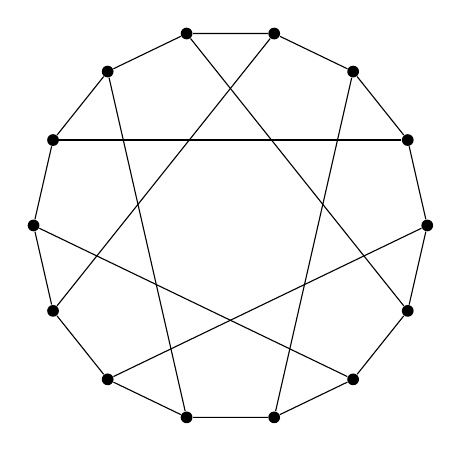
\begin{tikzpicture}[every node/.style={circle,fill=black,inner sep=1.5pt}, ->, >=stealth]
    
        % parameters
        \def\n{14}                   % number of vertices
        \def\radius{2.5cm}          % radius
        \def\startangle{90+360/28}         % start at top
        \def\step{360/\n}           % step angle

        % --- Nodes: start at top and descend clockwise ---
        \foreach \i in {0,...,13} {%
            \edef\nodename{v\i}%
            \node (\nodename) at ({\startangle - \step*\i}:\radius) {};%
        }

        \draw[-] (v0) -- (v1);
        \draw[-] (v1) -- (v2);
        \draw[-] (v2) -- (v3);
        \draw[-] (v3) -- (v4);
        \draw[-] (v4) -- (v5);
        \draw[-] (v5) -- (v6);
        \draw[-] (v6) -- (v7);
        \draw[-] (v7) -- (v8);
        \draw[-] (v8) -- (v9);
        \draw[-] (v9) -- (v10);
        \draw[-] (v10) -- (v11);
        \draw[-] (v11) -- (v12);
        \draw[-] (v12) -- (v13);
        \draw[-] (v13) -- (v0);
        \draw[-] (v0) -- (v5);
        \draw[-] (v1) -- (v10);
        \draw[-] (v2) -- (v7);
        \draw[-] (v3) -- (v12);
        \draw[-] (v4) -- (v9);
        \draw[-] (v6) -- (v11);
        \draw[-] (v8) -- (v13);
            
    \end{tikzpicture}
\end{center}

\end{proof}

\subsection*{Bonus}
Prove that the discrepancy of a $2$-regular hypergraph is at most 2.
\begin{proof}
Let $H=(V, \mathcal{E})$ be a 2-regular hypergraph. Let the dual graph be $G^*$. The vertices of $G^*$ are the edges of $H$ (the set $\mathcal{E}$). The edges of $G^*$ correspond to the vertices of $H$. Since every vertex $v \in V$ is contained in exactly two edges $e_i, e_j \in \mathcal{E}$, $v$ becomes an edge connecting node $e_i$ and node $e_j$ in $G^*$. $G^*$ is a standard multigraph. Now assign values $\Psi(e^*) \in \{-1, +1\}$ to the edges of $G^*$ (which are the vertices of $H$). The discrepancy of a hyperedge $e_j \in \mathcal{E}$ is the magnitude of the sum of the values of the edges incident to vertex $e_j$ in $G^*$. To minimize this, we can orient $G^*$. If we can orient $G^*$ such that for every vertex, the difference between in-degree and out-degree is small, we can assign $+1$ to incoming edges and $-1$ to outgoing edges. If $G^*$ is Eulerian (all degrees even), we can find an Eulerian tour and alternate directions. The net sum at every vertex is 0. Else, if $G^*$ has vertices of odd degree, we add a dummy vertex $z$ connected to all odd-degree vertices. The new graph is Eulerian. Thus, we can an Euler tour and orient it, then we can remove $z$. Now, consider some $u$ in $G^*$. If $u$ had even degree, it was not connected to $z$, so its balance is 0. If $u$ had odd degree, one edge (connecting to $z$) is removed. The remaining edges sum to $\pm 1$. Thus, the discrepancy is at most 1. Since $1 \le 2$, the discrepancy of a $2$-regular hypergraph is at most 2.
\end{proof}